\clearpage
\section{Architettura Skill}

L'architettura della skill che risiede in cloud in AWS Lambda è rappresentata dal seguente diagramma:

\begin{figure}[H]
	\begin{center}
		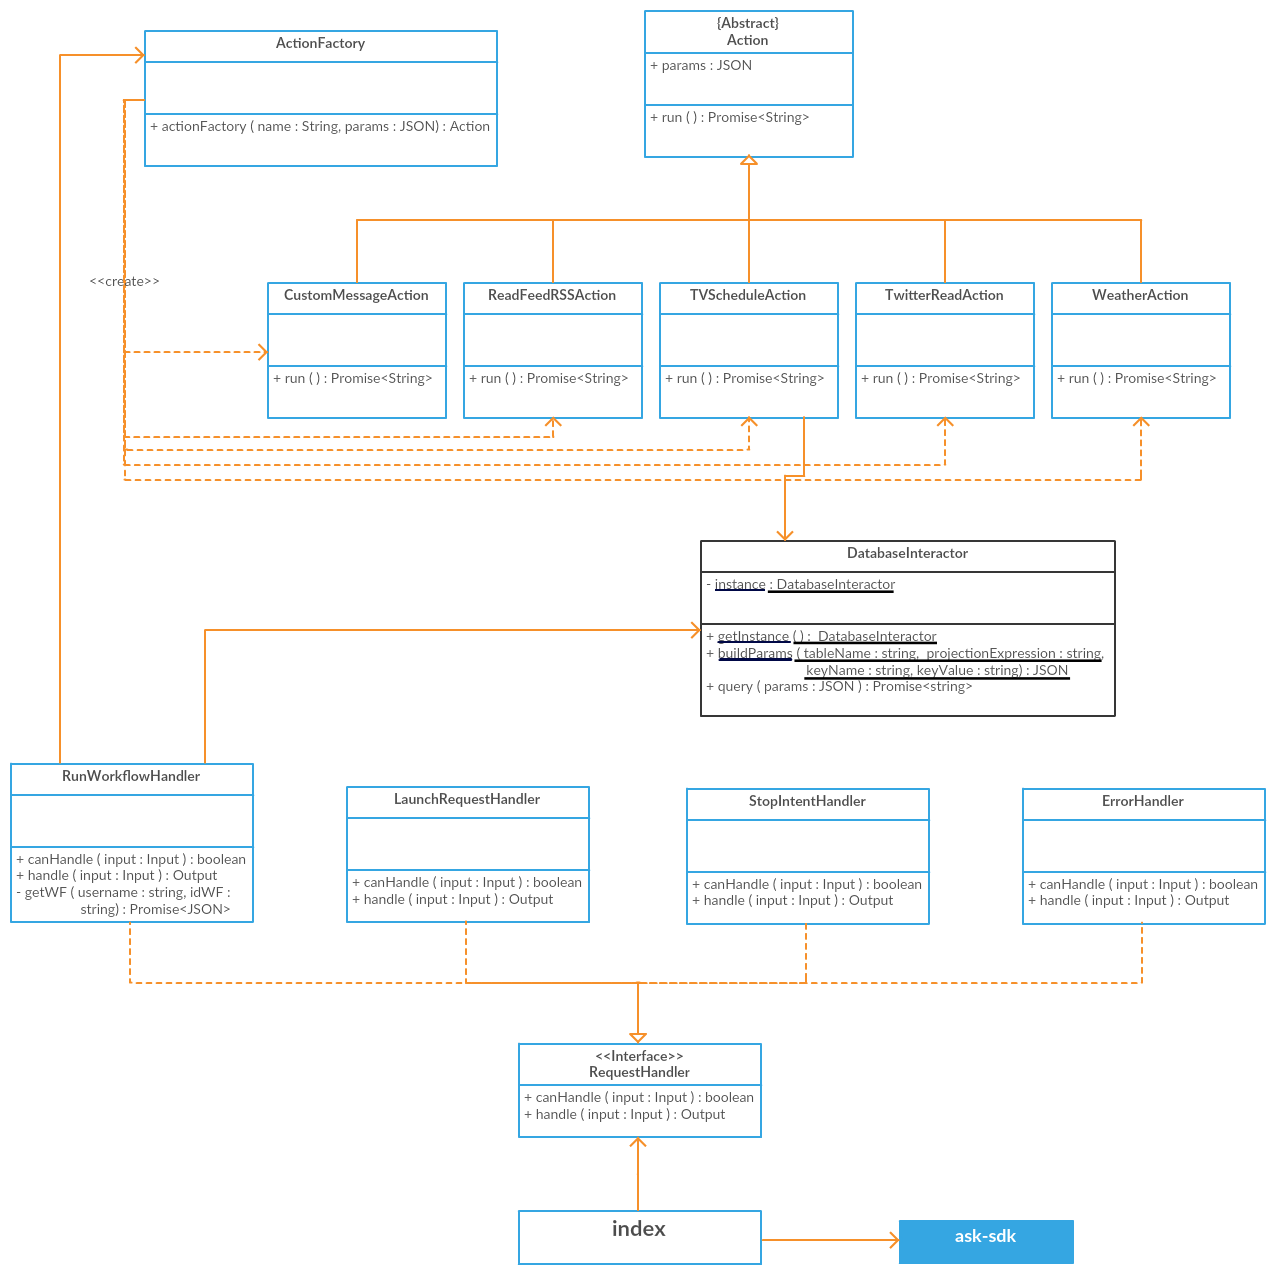
\includegraphics[width=\textwidth, keepaspectratio]{../includes/pics/Skill.png}
		\caption{Overview architetturale della skill.}
	\end{center}
\end{figure}
%TODO descrizione e dire che la struttura generale è visibile nella figura, aggiungere quindi il diagramma della skill completa

\subsection{Back-end}
La logica della skill è gestita dal file index.js al quale Alexa si appoggerà per l'invio delle richieste derivanti dall'interazione con l'utente.
Ogni richiesta inviata incapsula una serie di dati, quali il tipo di intent che la attiva e i parametri forniti dall'utente, denominati slot, e sarà gestita da uno degli handler presenti nel file index.js.
Per ognuno di questi verrà eseguito il metodo \textit{canHandle()} e, in caso di ritorno positivo, sarà lanciato il relativo metodo \textit{handle()}, interrompendo la ricerca dell'handler adeguato.
Nel caso in cui non venga trovato alcun gestore appropriato, la skill ha un comportamento non definito che porta al suo arresto improvviso; pertanto la best practice prevede l'implementazione di un handler di default che viene eseguito all'occorrenza di errori.

\subsubsection{Handler}
L'interfaccia RequestHandler è fornita dalle librerie di AWS incluse nel package.
Espone un metodo \textit{canHandle(input : Input)} che ritornerà un booleano: \textit{true} nel caso in cui l'handler che lo ridefinisce dovrà gestire la richiesta passatagli; \textit{false} altrimenti.
Nel caso di ritorno positivo, verrà eseguito il metodo \textit{handle(input : Input)} fornito dall'interfaccia; la sua ridefinizione dovrà elaborare la richiesta in input per poter fornire un ritorno \textit{Output} comprensibile da Alexa.
Gli handler sono strutturati con uno strategy pattern descritto nel seguente diagramma:

\begin{figure}[H]
	\begin{center}
		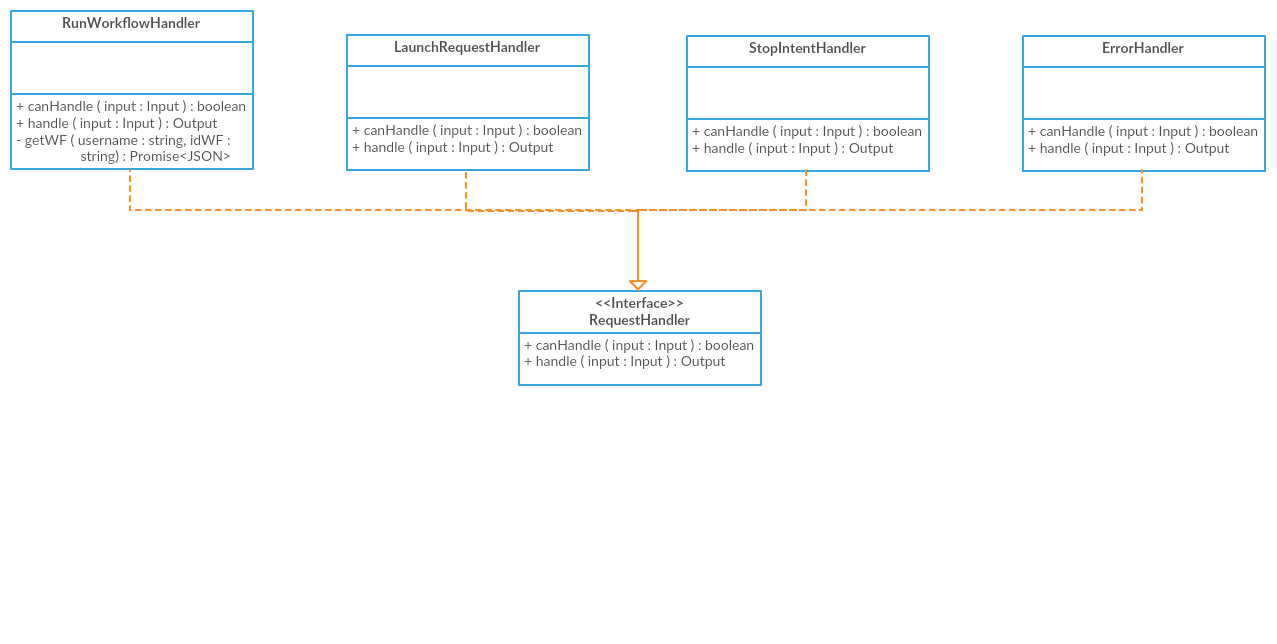
\includegraphics[width=0.9\textwidth, keepaspectratio]{../includes/pics/Strategy Pattern.png}
		\caption{Diagramma della classe Handler}
	\end{center}
\end{figure}


I principali handler da noi definiti sono:
\begin{itemize}
	\item \textit{LaunchRequestHandler}: gestisce il lancio iniziale della skill controllando che l'utente sia autenticato; in caso contrario lo invita ad effettuare il login con una notifica vocale e una push nell'applicazione Amazon Alexa dell'utente;
	\item \textit{RunWorkflowHandler}: viene lanciato quando l'utente richiede l'avvio di un workflow; si occupa di fare una query al database per ottenere i dati del workflow richiesto, quando disponibile, e cominciare la sua esecuzione;
	\item \textit{StopIntentHandler}: elabora la richiesta di arresto della skill da parte dell'utente;
	\item \textit{ErrorHandler}: è il gestore di default che verrà eseguito quando nessuno dei precedenti handler è stato avviato, o nel caso in cui si siano verificati errori durante l'esecuzione della skill;
\end{itemize}

\subsubsection{Action}
I workflow sono composti di azioni;
la loro struttura è definita da Action, questa è una classe astratta ed espone un metodo \textit{run()} che verrà chiamato per l'effettiva esecuzione dell'azione specifica.
La sua ridefinizione delinea il comportamento dell'azione concreta.\\
Le azioni ridefinite nella Skill SwetlApp sono:
\begin{itemize}
	\item \textit{CustomMessageAction}: consente ad Alexa di leggere un messaggio definito dall'utente;
	\item \textit{ReadFeedRSSAction}: consente ad Alexa di ricevere e leggere un feed rss impostato dall'utente;
	\item \textit{TVScheduleAction}: consente ad Alexa di informare l'utente sulla programmazione quotidiana dei suoi canali TV prefereriti;
	\item \textit{TwitterReadAction}: permette ad Alexa di leggere i tweet di un account Twitter definito dall'utente;
	\item \textit{TwitterWriteAction}: permette ad Alexa di postare un tweet personalizzato nella bacheca dell'utente;
\end{itemize}

\subsubsection{ActionFactory}
Si occupa della costruzione di un oggetto concreto di tipo derivante da Action.
Nasconde all'esterno il modo in cui viene scelto quale oggetto costruire, permette di estendere e manutenere velocemente e semplicemente il codice, in quanto per aggiungere una nuova Action sarà sufficiente che questa implementi l'interfaccia, e che venga aggiunto un controllo sul factory perchè questa sia usabile all'esterno.
Il controllo per capire qual è il tipo di azione corretto è fatto a partire dal nome dell'azione che viene chiesto come parametro, su questo sarà svolto uno switch case che ritorna l'azione corretta.

\begin{figure}[H]
	\begin{center}
		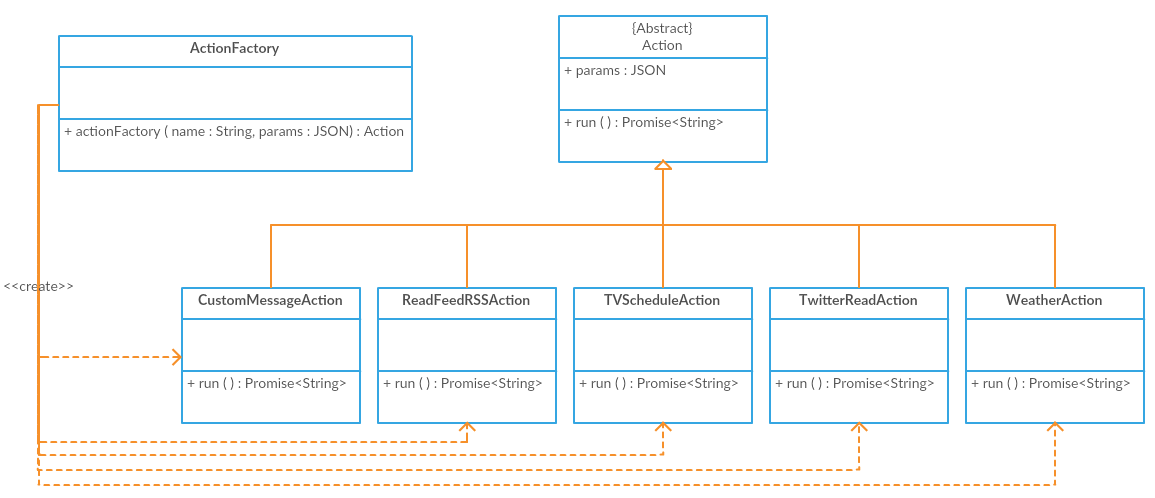
\includegraphics[width=0.9\textwidth, keepaspectratio]{../includes/pics/Factory Pattern.png}
		\caption{Diagramma della classe Action}
	\end{center}
\end{figure}

\subsubsection{Interazione con il database}
La connessione al db è gestita con un pattern singleton che quindi impone l'esistenza di un'unica istanza di \textit{DatabaseInteractor} in un dato momento. L'accesso di più client contemporaneamente al database è possibile perchè AWS si occupa poi di gestire le multiple richieste di accesso al db.
Fornisce un metodo di supporto \textit{query(params : JSON)} per gestire tutte le interazioni con il db direttamente da DatabaseInteractor.


\begin{figure}[H]
	\begin{center}
		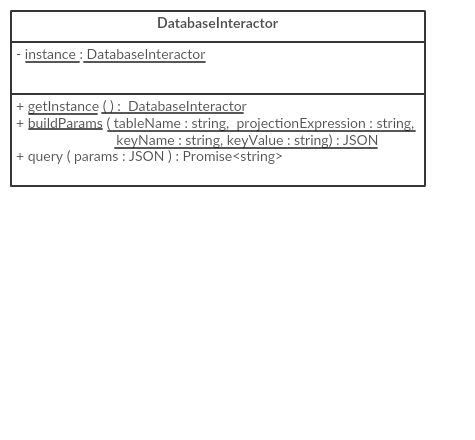
\includegraphics[width=0.75\textwidth, keepaspectratio]{../includes/pics/Singleton Pattern.png}
		\caption{Diagramma della classe DatabaseInteractor}
	\end{center}
\end{figure}
